\documentclass[a5paper, 10pt, twoside]{article}
\usepackage{import}
\usepackage{preamble}

\begin{document}

\begin{titlepage}
    \centering
    \topskip0pt
    \vspace*{\fill}
    
    {\sl\large Классы при механико-математическом факультете МГУ} \medskip

    {\sl\large Школа 54}

    \vspace*{4cm}

    \begin{spacing}{1}
        \LARGE\bfseries Записи лекций Летней Школы\par по Программированию
    \end{spacing}
    \smallskip
    
    {\Large С.\,С.\,Князевский}
    \vspace{.6cm}
    
    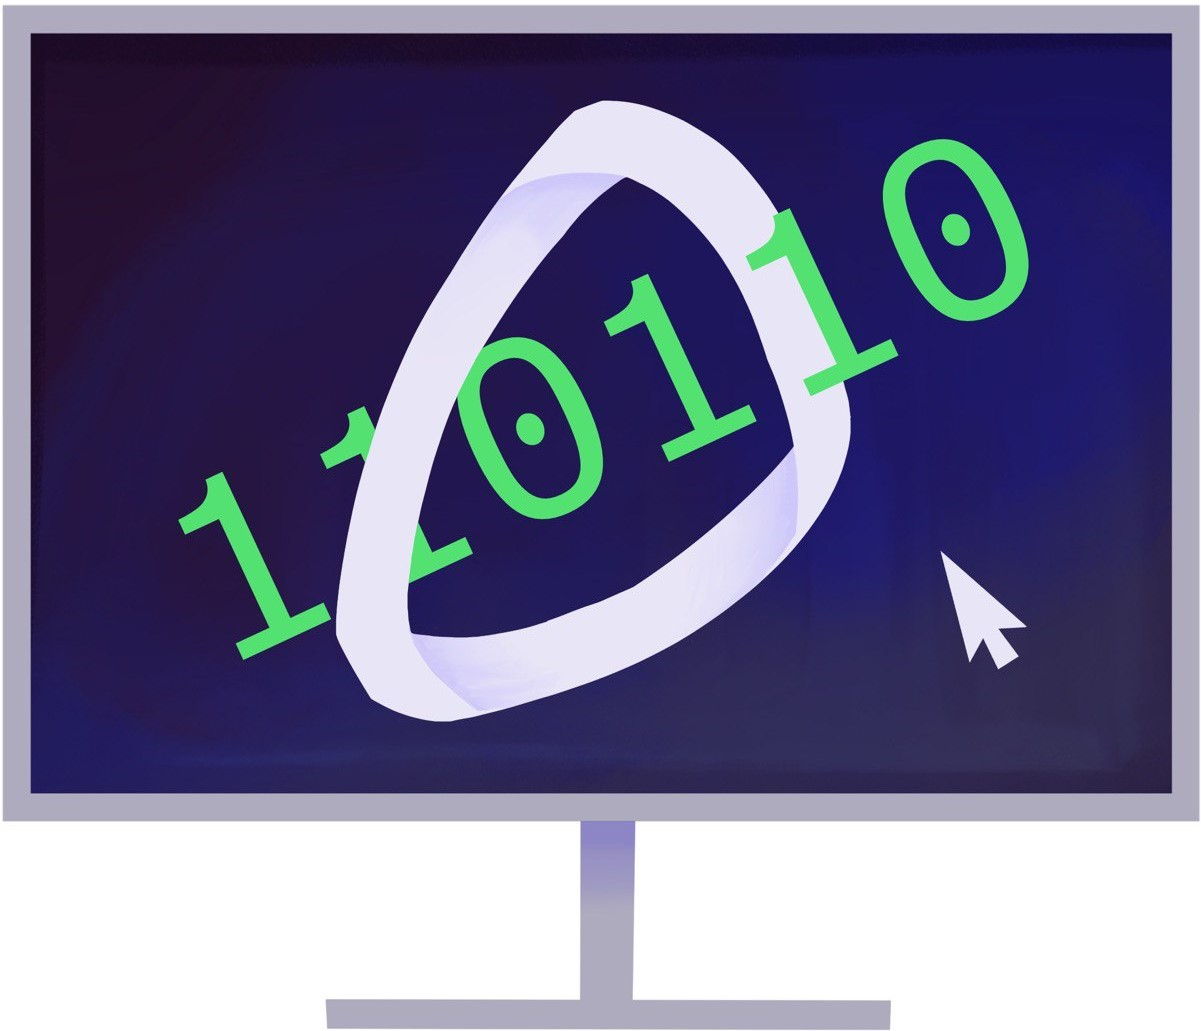
\includegraphics[width=0.4\textwidth]{img/logo.jpg}

    \vspace*{4cm}

    {\large Красновидово}\medskip
    
    {\large 10 --- 24 августа, 2024 год}
    \vspace*{\fill}
\end{titlepage}

\thispagestyle{empty}

\begin{abstract}
    Данные материалы являются конспектом лекций, прочитанных в Летней школе по программированию в 2024\,г. Сергеем Сергеевичем Князевским и студентами механико-математического факультета МГУ им. М.\,В.\,Ломоносова: Пшеничным Никитой, Клочковым Иваном и Хакамовым Рамилем. Представленные в данной брошюре темы были выбраны с целью подготовки к олимпиадам по программированию различного уровня, начиная со школьного и заканчивая всероссийским.

    Набор осуществлял Пшеничный Никита при участии Льва Целомудрова. За редактуру и вычитку спасибо Сергею Сергеевичу Князевскому.
\end{abstract}

\newpage

\tableofcontents
\newpage

\import{junior/}{linear_algos.tex}
\import{senior/}{sqrt_optimization.tex}
\import{junior/}{linear_structs.tex}
\import{senior/}{seg_tree.tex}
\import{junior/}{bfs.tex}
\import{senior/}{dsu.tex}
\import{junior/}{dfs.tex}
\import{senior/}{dyn_prog.tex}
\import{junior/}{short_paths.tex}
\import{junior/}{bits_opers.tex}
\import{senior/}{lca.tex}
\import{junior/}{stl.tex}
\import{senior/}{bridges.tex}
\import{junior/}{bin_search.tex}
\import{senior/}{strings.tex}
\import{junior/}{dyn_prog.tex}
\import{junior/}{math.tex}
\import{senior/}{fenwick.tex}

\newpage
\thispagestyle{empty}

% \noindent
% \topskip0pt
% \vspace*{\fill}
% 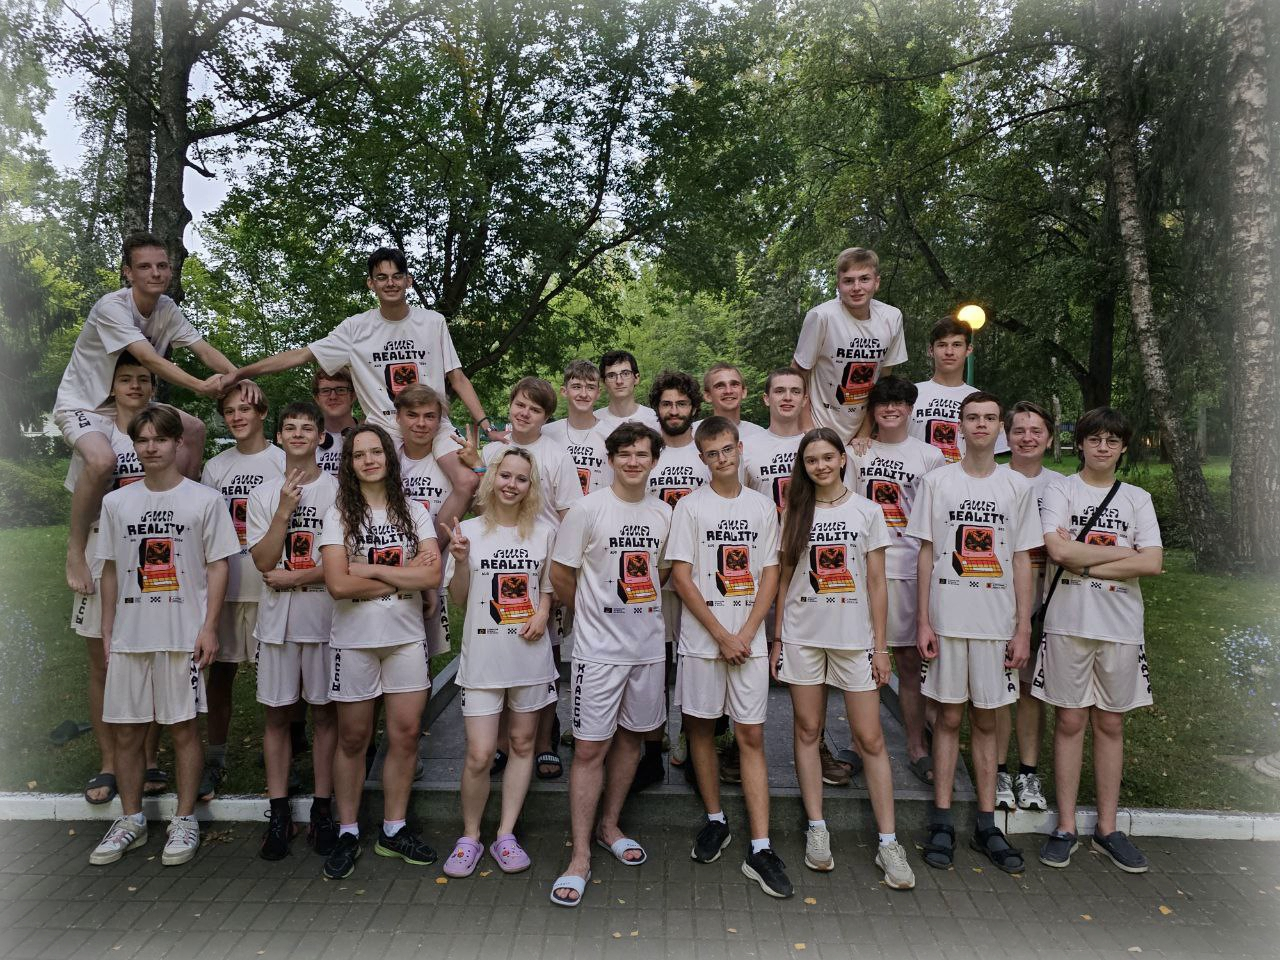
\includegraphics[width=\textwidth]{img/final_photo.jpg}
% \vspace*{\fill}

\end{document}
